\item \textbf{{[}ACJC/PRELIM/9569/2021/P1/Q2{]} }

The recursive function \texttt{Binomial} has two parameters, \texttt{N}
and \texttt{R}.

\noindent %
\noindent\begin{minipage}[t]{1\columnwidth}%
\texttt{01\qquad{}FUNCTION Binomial(N, R : INTEGERS) RETURNS INTEGER }

\texttt{02\qquad{}\qquad{}IF R = 0 OR R = N }

\texttt{03\qquad{}\qquad{}\qquad{}THEN }

\texttt{04\qquad{}\qquad{}\qquad{}\qquad{}Answer \textleftarrow{}
1 }

\texttt{05\qquad{}\qquad{}\qquad{}ELSE }

\texttt{06\qquad{}\qquad{}\qquad{}\qquad{}Answer \textleftarrow{}
Binomial(N \textendash{} 1, R) + Binomial(N \textendash{} 1, R \textendash{}
1) }

\texttt{07\qquad{}\qquad{}ENDIF }

\texttt{08\qquad{}\qquad{}RETURN Answer }

\texttt{09\qquad{}ENDFUNCTION}%
\end{minipage}
\begin{enumerate}
\item State what is meant by a recursive function, and identify the line
number that makes \texttt{Binomial} recursive. \hfill{}{[}2{]}
\item An example of a trace tree diagram showing the recursive function
call \texttt{Binomial(3,1)} is shown.
\begin{center}
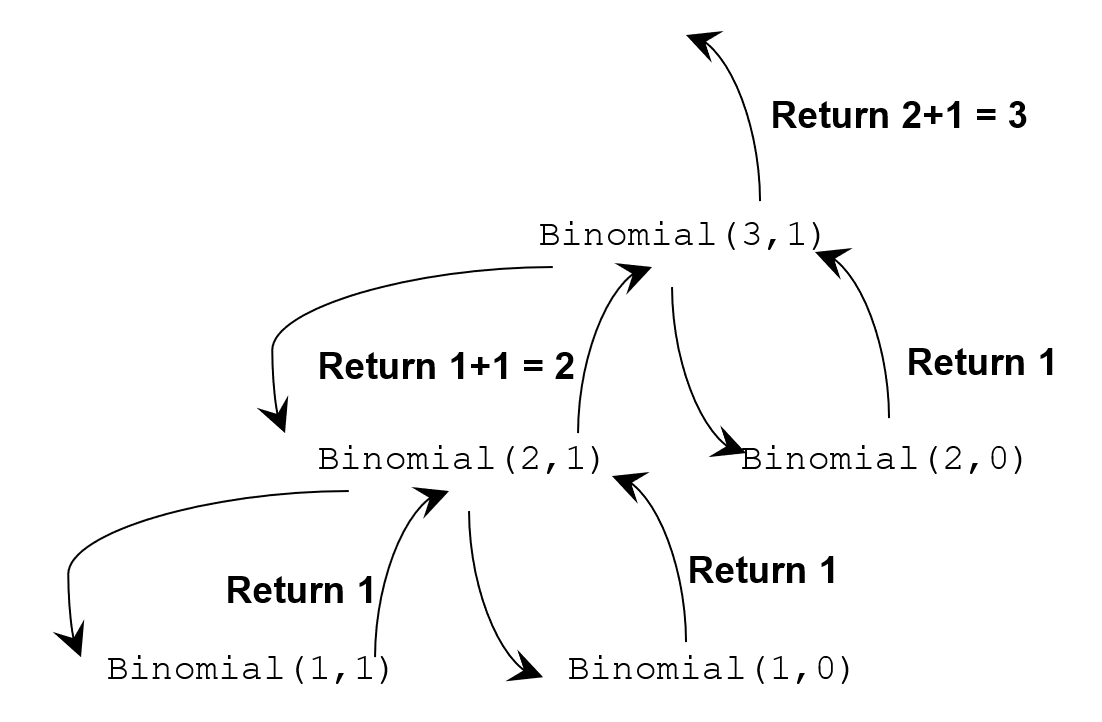
\includegraphics[width=0.5\paperwidth]{C:/Users/Admin/Desktop/Github/question_bank/LyX/static/img/9569-ACJC-2020-P1-Q2}
\par\end{center}

\end{enumerate}
Use the above example to create a trace tree diagram for the recursive
function call \texttt{Binomial(3,2)}. \hfill{}{[}4{]}
\begin{enumerate}
\item[(c)] Give values of N and R which would cause the function to enter infinite
recursion. \hfill{}{[}2{]}
\end{enumerate}